\section{Findings and results}
As an overview of the overall project, the resulting knowledge graph generated contains more than seven million of statements.
To imagine how big this graph could have become, it is worth remembering that only the information related with the artists, genres and locations from the original dataset was used to generate the graph.
Moreover, with respect of the MusicBrainz database, there exist more than twenty million of albums and tracks instances.

\begin{figure}[!tbh]
\centering
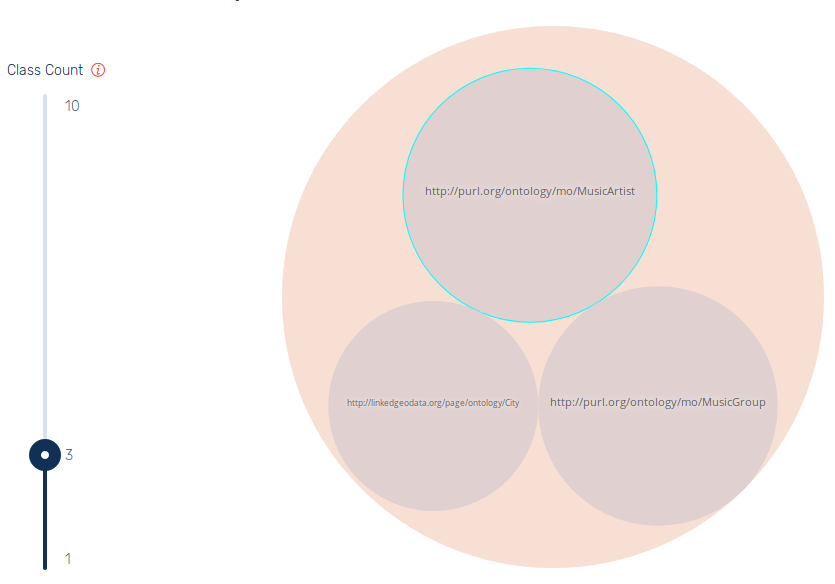
\includegraphics[width=0.8\linewidth]{images/classes}
\caption{Entity types with the greatest number of instances of the graph.}
\label{fig:classes}
\end{figure} 

Regarding the composition of the graph, entities of ten different classes exist, being \textit{MusicArtist}, \textit{MusicGroup} and City the three with more instances, figure \ref{fig:classes}. In the subfigure \ref{subfig:green_day}, a graphical example of the knowledge graph can be appreciated showing the information of a rather complete music group. The example shows most of the possible relations that can be found, having as the centre node a group band, it is related with some genres (yellow), their members and supporting musicians (purple) and the area it comes from (blue).

\begin{figure}[!tbh]
	\centering
	\begin{subfigure}{0.65\columnwidth}
		\centering
		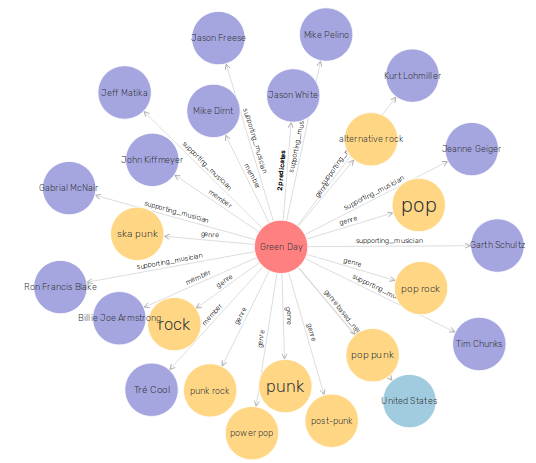
\includegraphics[width=0.7\linewidth]{images/greenday.png}
		\caption{Green Day information in the knowledge graph.}
		\label{subfig:green_day}
	\end{subfigure}
	\begin{subfigure}{0.30\columnwidth}
		\centering
		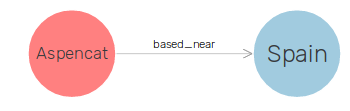
\includegraphics[width=0.63\linewidth]{images/aspencat.png}
		\caption{Aspencat information in the knowledge graph.}
		\label{subfig:aspencat}
	\end{subfigure}

	\caption{Comparison between \textbf{a.}known and commercial artist and \textbf{b.}alternative artist.}
	\label{fig:graph-comp}
\end{figure}

After the analysis of the knowledge graph, one of the findings that confirms the belief of the alternative groups having less complete information in these open platforms can be appreciated in figure \ref{fig:graph-comp}.
It is clear that, comparing the information presented in the subfigure \ref{subfig:green_day} with respect the subfigure \ref{subfig:aspencat}, the first is much more complete whereas in the second only the origin area is shown. 

Other aspect worth discussing in this section are the results obtained in the interlinking and completion tasks.
During the development of this phase, two opposed situations were found.
On the one hand, the work made with respect to the musical genres was successful and returned great results.
For example, from the original 419 genres contained in MusicBrainz, 368 were linked with Wikidata and 291 with DBpedia, meaning a success superior to the 70\% in both cases.

The previous situation was repeated for the completion of the genres, were 1217 of the 1568 original Wikidata genres were added and 389 of the 1245 of the DBpedia ones. 
These cases were favoured due to the use of a clear and stable set of definitions for the entities. 

On the other hand, the interlinking and completion tasks that were related to the artists and the areas did not turn that well.
Two reasons lead to these results, the entity definitions used in both sources to refer to music artists and the existence of different entities with the same name.  

Regarding the first situation, in the case of Wikidata, a music artist can have a wide range of types as its class definition due to the use of genres in them. 
For example, a music group like ``Green Day'' is defined like a \textit{rock band} whereas another similar band like ``blink-182'' is defined only like a \textit{band}.
This difficult greatly the possibility of generating a generalized way to complete the data among graphs, as the queries became very specific. 

The second situation\footnote{More details can be found in: \url{https://github.com/adrigrillo/music_kg/issues/8\#issuecomment-477783435}} is impossible to avoid due to the fact that a name cannot be considered a unique id for the different entities.
This kind of case can be solved with the use of more information related to the artist, like the year of foundation (\textit{7\_db\_relate-artist-genres-year.txt}).
However, this can be problematic when some of the data is missing in one of the datasets, or directly, in both, as there is no way to validate the relation.

\begin{figure}[!tbh]
	\centering
	\begin{subfigure}{0.49\columnwidth}
		\centering
		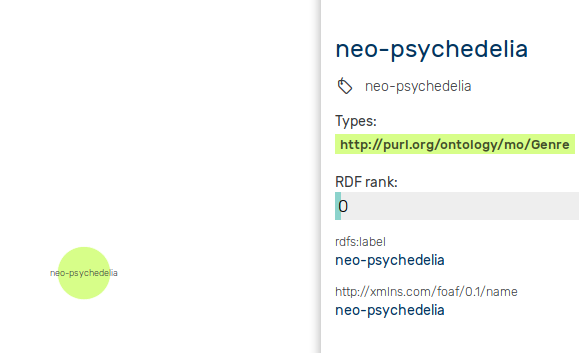
\includegraphics[width=0.7\linewidth]{images/neo-psychedelia.png}
		\caption{Before the completion task.}
		\label{subfig:before}
	\end{subfigure}
	\begin{subfigure}{0.49\columnwidth}
		\centering
		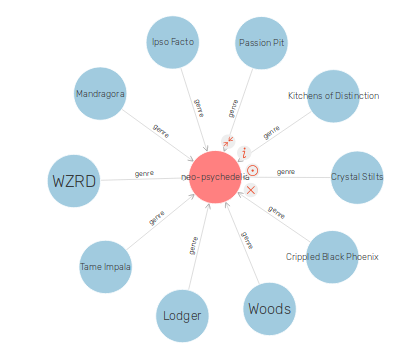
\includegraphics[width=0.63\linewidth]{images/neo-after.png}
		\caption{After the completion task.}
		\label{subfig:after}
	\end{subfigure}
	\caption{Information of genre before and after the completion task that relates artist with the new genres.}
	\label{fig:completion}
\end{figure}

As an example, the query that used the year of foundation correctly linked 1385 artist with the new genres, completing the graph as can be seen in figure \ref{fig:completion}, but the number is low compared with the million of artist present in the graph. 

Consequently, both of the described situations lead to the specialization of the queries in order to achieve correct results and moves them away of the objective of finding a generalized way to complete knowledge graphs. Moreover, this finding could be one of the reason because there is not much development in this topic. 